%!TEX root = ../thesis.tex

\chapter{Preliminaries}
\label{chap:prelim}
\section{Setting and Notations}
\subsection{Classification} 
\label{subsec:class}
\par  In this thesis we will mostly be concerned with \textit{classification}\cite{Hastie2009}. We have a, usually finite, set of labels denoted as $Y:=\set{y_1,\ldots y_n}$ and for a given input, which we will denote by $X$, we are expected to pick one of the labels to attach to it. Going back to our spam example this would look like $Y=\set{spam, genuine}$. As with this example it is useful to note that these labels usually lack any kind of structure like an order or magnitude, even though they are usually labelled with integers. In the case that we have only two labels they will often be labelled as 0 and 1 or 1 and -1. Which one is used usually depends on the algorithm. 

\par We will use upper case letters to denote generic instances of a variable while observed instances will be denoted by lower case letters. Vectors will be denoted in boldface and their components by subscripts. For example: $x_i$ is the $i$th instance of an observed input variable $X$, which may or may not be a vector again and $y_i$ it's label, which may or may not be known.  Predictions will be denoted by $\hat Y$, so in the case we have a hypothesis $h:X\to Y$ we will define $\hat{y_i}:=h(x_i)$. Generally any operation written using vectors, which may or may not be formally defined, is used to mean component wise operations. 

\subsection{Weak learning}
\label{subsec:weak}
In this thesis we will often refer to a class of algorithms called \textit{weak probably approximately correct(PAC) learning algorithms}\cite{Freund1997}. For conveniences' sake these algorithms will simply be referred to as ``weak learners'', and we will use \weak to denote a generic weak learning algorithm. These algorithms must satisfy the following conditions: given some $\delta,\gamma >0$ and access to enough examples these algorithms must output an hypothesis that has error at most $\ve \leq \frac12-\gamma$, with probability $1-\delta$. This means that the algorithm must, with a certain probability(the P in PAC), provide an hypothesis that performs at least slightly better than random guessing(the AC in PAC). 

\par In this thesis this role will mostly be fulfilled by what we call \textit{decision stumps}. These are decision trees of depth one. These usually operate in the following matter. Given an input vector $X$ the stump will attempt to find an optimal $t$ and $i$ such that the hypothesis $h:X\to Y$ given by $$h(x):=\begin{cases}1 &\text{if }x_i\leq t \\ -1 &\text{otherwise}\end{cases}$$ has minimal error on our (weighted) training set. Here we have chosen to check whether $x_i\leq t$ instead of $x_i\geq t$ but this is another choice for which the stump can optimize. 
\newpage
\subsection{Boosting}
\label{subsec:boost}

Let us give a more detailed description of the process of boosting. Firstly we require a set of training data and one weak learning algorithm \weak. Often a boosting algorithm will also accept a distribution $D$ on the training data to exploit any prior knowledge which will be set to uniform if no prior knowledge is provided. The procedure for each iteration is to fit \weak on our training data which produces an hypothesis $h^t:X\to Y$. Using this hypothesis we will calculate a loss vector we will denote with $\ell^t$. This loss vector is a measure for how well we have done and is usually some form of the error of \weak on the training set. For example \adaN will use a measure called the $\ve$-regret which will define in section \ref{sec:adaN}. Using this loss vector we will slightly alter the training set by attaching weights to them, which measure their importance and then repeat the process. This will give us a sequence of hypotheses which increasingly focus on the relevant examples.
\par When comparing algorithms, say for example we are comparing a algorithm $A$ to some simple procedures $\pi_i$, we will talk about the net-loss, often referred to as the \textit{regret}, of $A$ which is denoted $$R_A:=L_A-\min_i L_i$$ where $L_A$ this the loss of $A$ and $L_i$ is the loss of $\pi_i$. So when we talk about the regret we refer to the difference in loss we could have attained had we simply followed the best $\pi_i$, which we obviously want to minimize.

\section{AdaBoost}
\label{sec:ada}
\subsection{The algorithm}
\label{subsec:algo}
We will now give a formal discussion of the \adaB\cite{Freund1997} algorithm, which can be found in the appendix \ref{app:adaB}. The goal of the algorithm is to minimize the error with the respect to the distribution $D$ over the training data. One should note there that $D$ is initially provided to the learner but after that the learner can manipulate $D$ itself to minimize the error. In the first step the learner will obtain a new distribution by normalizing the weights from the previous step, or from the initial distribution. This distribution will then be provided to \weak which will form a hypothesis accordingly. When the hypothesis is formulated the learner will calculate it's error and set the parameter $\beta$, which can be interpreted as the learning speed. In the final step the learner will update the weights appropriately. It is important to observe that \weak produces an hypothesis at every iteration and that the final hypothesis is essentially a weighted majority vote among all of these hypotheses. 


\subsection{The theoretical performance of \adaB}
\label{subsec:perf}
Here we will discuss the theoretical performance of \adaB. One of the main results from \cite{Freund1997}, is the following theorem: 
\begin{theorem}\label{thm:adaErr}\cite{Freund1997}
Suppose the weak learning algorithm \weak when called by \adaB generates hypotheses with errors $\ve_1\ldots, \ve_T$ (as defined in step 3 in \ref{app:adaB}). Then the error \\$\ve:=\Pr_{i\sim D}[h_f(x_i)\neq y_i]$ of the final hypothesis $h_f$ output by \adaB is bounded above by $$\ve\leq 2^T\prod^T_{t=1}\sqrt{\ve_t(1-\ve_t)}$$
\end{theorem}
We will omit the proof since it is not the focus of this thesis but we will briefly discuss its consequences. As discussed above one might find it strange that every hypothesis is allowed a vote in the final hypothesis. This is still, however, an improvement over previous algorithms since the final error will now depend on the error of all hypotheses instead of only the worst, as was the case in previous works. It is also not immediately obvious that this upper bound does us any good since it contains exponents and products for which it is not trivial how they cancel out. In their paper Freund and Shapire reduce the above stated upper bound to the following one: $$\ve\leq \exp\left(-2\sum^T_{i=0}\gamma_t^2\right)$$ where the $\gamma_t$ is defined such that $\ve_t=1/2-\gamma_t$ holds. This upper bound is more useful since it decreases exponentially, leading us to conclude that \adaB has a good theoretical performance.   

\subsection{The practical performance of \adaB}
\label{subsec:pracPerf}
In an attempt to demonstrate the practical performance we recreated the following situation from \cite{Hastie2009}. We have ten features $X_1,\ldots,X_{10}$ which are drawn from a standard independent Gaussian. Their label is determined (deterministically) by the following rule: $$Y:=\begin{cases}
1 & \sum_{k=0}^{10} X^2_k > \chi_{10}^2(0.5)\\
0 & \text{otherwise}
\end{cases}$$ Where $\chi_{10}^2(0.5)=9.34$ is the median of a chi-squared random variable with ten degrees of freedom. The results of testing can be found in figure \ref{fig:adaB} and will be discussed below. 

\begin{figure}[!ht]
  \centering
      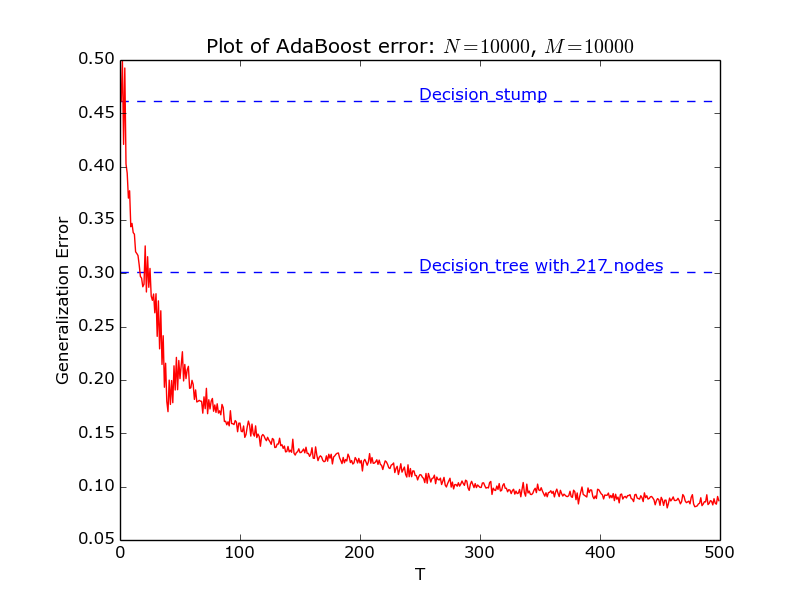
\includegraphics[width=0.8\textwidth]{generated/longCorrect.png}
  \caption{Generalization error of AdaBoost as a function of number of iterations with 10000 examples and test cases. The error of actual stumps and a tree with 217 nodes is also shown for reference}
      \label{fig:adaB}
\end{figure}

First of all it should be noted that we took an equal amount of training and testing examples (10000 to be exact). This is was possible because we can generate the data ourselves in a reasonable amount of time. In practical settings this is however usually not the case and one would need to reserve a portion of their data for testing instead of training. This means that the more testing one does, the less training one can do an thus, generally one would reserve only around 10\% of their data for testing.
\par Looking at figure \ref{fig:adaB} it is obvious that our algorithm works. The decision stump initially performs with an error rate of 47\% which is indeed only just better than random guessing. \adaB outperforms this and even a large tree with 217 nodes and an error rate of 30\% after just tenths of iterations and reaches an error rate as low as 8\% after 400 iterations. 
\todo[line]{Mocht er genoeg tijd zijn dan wil ik hier een stuk invoegen over de rekentijd van \adaB }

\section{\adaN}
\label{sec:adaN}
In their paper \cite{Luo2014} Luo and Schapire use their analysis to develop \textbf{NormalHedge.DT} which they apply to form the algorithm they